\documentclass[preprint, 3p,
authoryear]{elsarticle} %review=doublespace preprint=single 5p=2 column
%%% Begin My package additions %%%%%%%%%%%%%%%%%%%

\usepackage[hyphens]{url}

  \journal{Energy Economics} % Sets Journal name

\usepackage{graphicx}
%%%%%%%%%%%%%%%% end my additions to header

\usepackage[T1]{fontenc}
\usepackage{lmodern}
\usepackage{amssymb,amsmath}
% TODO: Currently lineno needs to be loaded after amsmath because of conflict
% https://github.com/latex-lineno/lineno/issues/5
\usepackage{lineno} % add
\usepackage{ifxetex,ifluatex}
\usepackage{fixltx2e} % provides \textsubscript
% use upquote if available, for straight quotes in verbatim environments
\IfFileExists{upquote.sty}{\usepackage{upquote}}{}
\ifnum 0\ifxetex 1\fi\ifluatex 1\fi=0 % if pdftex
  \usepackage[utf8]{inputenc}
\else % if luatex or xelatex
  \usepackage{fontspec}
  \ifxetex
    \usepackage{xltxtra,xunicode}
  \fi
  \defaultfontfeatures{Mapping=tex-text,Scale=MatchLowercase}
  \newcommand{\euro}{€}
\fi
% use microtype if available
\IfFileExists{microtype.sty}{\usepackage{microtype}}{}
\usepackage[]{natbib}
\bibliographystyle{elsarticle-harv}

\ifxetex
  \usepackage[setpagesize=false, % page size defined by xetex
              unicode=false, % unicode breaks when used with xetex
              xetex]{hyperref}
\else
  \usepackage[unicode=true]{hyperref}
\fi
\hypersetup{breaklinks=true,
            bookmarks=true,
            pdfauthor={},
            pdftitle={European Carbon Market Connectedness and Risk Contagion: A Study of Return and Volatility Dynamics Between European Union Allowances (EUAs) and Financial Markets post-Fit for 55 and RePowerEU},
            colorlinks=false,
            urlcolor=blue,
            linkcolor=magenta,
            pdfborder={0 0 0}}

\setcounter{secnumdepth}{5}
% Pandoc toggle for numbering sections (defaults to be off)


% tightlist command for lists without linebreak
\providecommand{\tightlist}{%
  \setlength{\itemsep}{0pt}\setlength{\parskip}{0pt}}




\usepackage{subcaption, float, adjustbox}



\begin{document}


\begin{frontmatter}

  \title{European Carbon Market Connectedness and Risk Contagion: A
Study of Return and Volatility Dynamics Between European Union
Allowances (EUAs) and Financial Markets post-Fit for 55 and RePowerEU}
    \author[cisl,sigma]{Carlos Arcilla Barrera%
  %
  }
   \ead{ca577@cantab.ac.uk} 
    \author[cam]{Emre Usenmez%
  \corref{cor1}%
  }
   \ead{eu229@cam.ac.uk} 
      \affiliation[cisl]{
    organization={University of Cambridge Institute for Sustainability
Leadership},addressline={1 Regent Street},city={Cambridge},postcode={CB2
1GG},country={UK},}
    \affiliation[sigma]{
    organization={Sigma Advanced Capital Management},addressline={203
North LeSalle Dr, Suite
2110},city={Chicago},postcode={60601},country={USA},}
    \affiliation[cam]{
    organization={Gonville \& Caius College, University of
Cambridge},addressline={Trinity Street},city={Cambridge},postcode={CB2
1TA},country={UK},}
    \cortext[cor1]{Corresponding author}
  
  \begin{abstract}
  This paper uses Diebold-Yilmaz model to analyze the return and
  volatility connectedness between the European carbon market and the
  financial markets from the commencement of the 3rd phase of the EU
  emissions trading system in 2013 to August 2024 in order to ascertain
  the impact of both exogenous shocks and the recent reforms introduced
  under the Fit for 55 package and RePowerEU Plan. We examine the static
  and dynamic characteristics of the connectedness network and find that
  the return and volatility behavior of the European carbon market are
  primarily driven by their own fundamental factors, thus largely
  independent of other financial markets, except for coal and natural
  gas, and except during periods of financial stress where a relatively
  short-lived increase in the connectedness with other financial markets
  is observed.
  \end{abstract}
    \begin{keyword}
    Carbon markets \sep emissions trading system \sep connectedness
measures \sep 
    system risk
  \end{keyword}
  
 \end{frontmatter}

\hypertarget{introduction}{%
\section{Introduction}\label{introduction}}

In the late 19th century the Swedish scientist Svante Arrhenius
discovered\footnote{Building on the works of Joseph Fourier and John Tyndall roughly half a century earlier \citep{corfee-morlot_global_2007}}
the link between increases in carbon dioxide (CO2) concentrations in the
atmosphere, fossil fuel burning, and the greenhouse effect
\citep{corfee-morlot_global_2007, hart_scientific_1993, weart_discovery_2008}.
A century and a quarter later, in 2022, emissions worldwide have been
recorded at 57.4 gigatons of carbon dioxide equivalent (GtCO2e), with
the energy sector accounting for a little over third of these at 20.9
GtCO2e and industry another quarter at 14.4GtCO2e
\citep{unep_emissions_2023}.

As one of the top polluters \citep{unep_emissions_2023}, the European
Union (EU) has established an ambitious climate objective of 55\%
reduction in greenhouse gas emissions (GHGs) by 2030 from the 1990
levels \citep[Art 4(1)]{regulation_2021_1119}. To ensure the feasibility
of this objective, the European Commission (EC) has adopted a
comprehensive suite of legislative changes under Fit for 55 package
within a broader sustainable growth strategy under the European Green
Deal \citep{delivering_2021}.

In parallel to its decarbonization efforts, the EU also launched
RePowerEU Plan in 2022, a strategic response to the energy crisis
triggered by Russia's invasion of Ukraine in that year
\citep{communication_2022}. This plan aims to reduce the EU's dependency
on Russian fossil fuels by significantly accelerating the transition to
renewable energy sources, enhancing energy efficiency, and diversifying
the EU's energy supply chains \citep[1-5]{communication_2022}.

Under Fit for 55, the EC has proposed a set of reforms to the EU
emissions trading system (EU ETS) which have duly been adopted by the
European Commission in May 2023 \citep{directive_2023_959}. The EU ETS
itself is one of the central instruments of the EU in its
decarbonization and energy transition efforts
\citep{decision_2015_1814, bai_drivers_2023}, and it currently covers
about 40\% of the EU's GHG
emissions\footnote{The coverage will likely increase after the reforms are transposed into national laws of member states by 30 June 2024 \citep{directive_2023_959}}
\citep{eu_ets}. Under this mechanism a European Emission Allowance (EUA)
is a permit granting the right to emit one ton of CO2 which can then be
traded \citep{directive_2003_87}.

The EU ETS has evolved over four phases. The first phase, covering the
period from 2005 to 2007, has essentially established the market
mechanism underpinning the EU ETS \citep[Art. 11(1)]{directive_2003_87}.
The second phase, covering the five-year period from 1st of January
2008, has imposed a more stringent cap on the Union-wide total EUAs but
the mechanism still ended up with surplus of allowances largely due to
the 2008 recession \citep{ellerman_eu_2014, bel_emission_2015}. With the
commencement of the third phase on 1 January 2013, there has been a
shift from national allocation
plans\footnote{During the phases I and II of the EU emissions trading system (EU-ETS), each EU country decided on the allocation of their emission allowances. \citep[Art. 11]{directive_2003_87}}
to an EU-wide cap in the total number of
allowances\footnote{The total number of annual allowances also decrease by a linear factor of 1.74 percent. To address the surplus allowances that have been accumulating since Phase II, a new market stability reserve (MSR) has additionally been introduced that acts as a repository for excess portions of auctionable allowances and replenishes the market if allowances in circulation are fewer than 400 million \citep{decision_2015_1814, simoes_revision_2022}}
\citep[Art. 1]{directive_2009_29}. The fourth and current phase that
started in 2021, and will continue until 2030, has further reduced the
EU-wide allowance cap with more stringent rules for free
allocation\footnote{It also increased the annual reduction factor to 2.2 percent and earmarked a portion of MSR for innovation support.}
\citep{directive_2018_410}. In parallel, the Fit for 55 package has,
among other initiatives, extended the scope of the ETS to include
emissions from shipping and has accelerated the reduction of both the
free allocations and the total allowances within Phase
IV\footnote{This was done by increasing the linear reduction factor from 2.2 percent to 4.2 percent starting in 2024.}
\citep{directive_2023_959}.

The effectiveness of the EU ETS in decarbonizing and facilitating the
energy transition depends on several factors
\citep{backe_exploring_2023, de_cara_marginal_2011, marin_impact_2018, scheelhaase_options_2021}.
Among these factors, the price of EUAs plays a critical role
\citep{pietzcker_tightening_2021, quemin_raising_2022, lovcha_determinants_2022}.
Higher EUA prices have the potential to drive significant
transformations across multiple sectors, encouraging firms to innovate
and reduce emissions \citep{pietzcker_tightening_2021, recka_2015}. Such
realization of higher EUA prices can be aided by increased participation
of financial institutions which can promote liquidity, price discovery,
transparency, and improved market efficiency
\citep{bohl_impact_2023, corgnet_information_2021}. This in turn
depends, among other factors, on the price volatility which can raise
uncertainty and restrain investment into carbon-reducing technologies
\citep{acworth_emissions_2017, laing_assessing_2013}.

This study, therefore, analyzes, via return and volatility
connectedness, the degree of integration of EUAs with other asset
classes to assess potential diversification benefits EUAs may offer. If
present, such diversification benefits can consequently incentivize
increased participation by financial institutions and help the EU's
efforts in decarbonization and transitioning into renewables.
Accordingly, this study contributes to the literature on energy and
sustainable finance as well as on risk management in three complementary
ways. First, carbon is treated as an independent asset class whereas
previous works largely examine the issue within an energy context. To
the best of our knowledge, this is the first time it is treated as such
while incorporating the changes emerging from the Fit for 55 package and
RePowerEU. Within this context, this study considers return and
volatility spillovers within a broader range of markets, ranging from
fixed income and European and US equities to commodities. Second, while
the existing literature largely considers Phases I to III of EU ETS,
this study also incorporates Phase IV providing a more comprehensive
analysis of the recent changes. Third, market stress periods -- such as
Covid-19 and the Russian-Ukrainian War -- are uniquely considered in
analyzing the changes in EU ETS connectedness and its integration with
other asset classes over time.

Three key results emerge from this study. First, we find that EUAs show
stronger connection with other financial markets mainly during periods
of financial crises. However, aside from connectedness with coal and
natural gas markets, these connections tend to be short-lived, and EUAs
generally remain independent. Second, our results indicate that the
European carbon market tend to be a net receiver of return and
volatility spillovers, suggesting that external factors influence this
market more than carbon-specific factors influence other markets. Third,
it appears that to date the reforms introduced by the Fit for 55
package, RePowerEU, and Phase IV may not have exerted as strong an
impact as market stresses, although it seems that their impact may have
a longer duration.

The rest of the paper is as follows. The next section provides a
literature review of the related studies. Section 3 specifies the
methodology and Section 4 describes the data. Section 5 presents the
main empirical findings and discussion, and Section 6 provides our
concluding remarks and implications.

\hypertarget{literature-review}{%
\section{Literature Review}\label{literature-review}}

Since the EU ETS has come into force, empirical literature on carbon
trading mechanisms has mainly focused on its price dynamics, on its
impact on the economy, and its relationship with various markets along
with its hedging benefits
\citep{demiralay_carbon_2022, dai_impact_2022}.

Ability to accurately forecast carbon prices are important in enabling
decisions on emissions and transition tradeoffs
\citep{wang_novel_2021, zhang_forecasting_2024, chen_multiscale_2024}.
To that end, while some have considered the role of attention in carbon
pricing
\citep{zheng_relationship_2022, gong_climate_2023, zhang_forecasting_2024},
some have used VAR \citep{arouri_nonlinearities_2012}, ARIMA
\citep{garcia-martos_modelling_2013}, GARCH
\citep{byun_forecasting_2013} and its modifications including, among
others, stable-Paretian-GARCH \citep{paolella_econometric_2008}, Markov
switching GARCH \citep{benz_modeling_2009},
VMD-GARCH\citep{huang_hybrid_2021}, switching transition regression
exponential GARCH \citep{arouri_nonlinearities_2012}, and AR-GARCH
\citep{benz_modeling_2009} to capture volatility, skewness, and excess
kurtosis. Yet others have looked at the impact of fuel switching on
carbon prices
\citep{bertrand_carbon_2014, hintermann_allowance_2010, pettersson_fuel_2012},
while some others at the impact of policy uncertainties on the
volatility of carbon markets \citep{dai_impact_2022, dong_extreme_2024},
and some have used various decomposition and artificial intelligence
techniques to improve the forecasting ability
\citep{QIN2024131410, wang_novel_2021, chen_multiscale_2024}. What is
evident is that it is a challenge to forecast carbon prices since they
are nonstationary and show nonlinearity, and it is likely that the
information shocks transmit between different markets
\citep{feng_carbon_2011, lutz_nonlinearity_2013, segnon_modeling_2017, chen_multiscale_2024}.

Emissions trading can help in reducing the abatement costs and dampen
the negative impact of emission reductions on GDP
\citep{wu_achieving_2016, lin_impacts_2019}, although some of the carbon
reduction gains may decline overtime due to macroeconomic carbon rebound
effect \citep{bolat_is_2023}. Its impact on the economy, though, mainly
has a sectoral perspective. Within that perspective, the predominant
focus is on its strong impact on the energy industry
\citep{delarue_simulating_2007, kara_impacts_2008, zachmann_first_2008, kirat_impact_2011, bonenti_evaluating_2013, hobbie_windfall_2019, hanif_nonlinear_2021, dai_impact_2022},
and, to a lesser extent, on its negligible impact on the aviation,
cement, steel, and aluminum sectors
\citep{VANASSELT2007497, zhang_overview_2010, oberndorfer_costs_2007, efthymiou_eu_2019}.

There also appears to be a positive relationship, albeit in varying
degrees, between carbon markets on the one hand and equities, oil,
natural gas, coal, and electricity prices on the other
\citep{mansanet-bataller_co_2007, alberola_price_2008, keppler_causalities_2010, bredin_emerging_2011, chevallier_evaluating_2011, creti_carbon_2012, aatola_price_2013, zhang_dynamic_2016, ji_information_2018, falbo_renewables_2019, fiori_energy_2024}.
However, with the changes introduced in each of the subsequent phases
such impacts became harder to establish
\citep{arouri_nonlinearities_2012, wu_market-linkage_2020}.
Nevertheless, there is likely a stronger relationship between carbon and
energy assets compared to financial assets for the duration of Phase II
and most of Phase III, which, for a non-energy portfolio, may provide
some diversification benefits
\citep{tan_how_2020, lovcha_determinants_2022, yang_idiosyncratic_2022}.
Moreover, interconnectedness of the carbon with other markets evolves
overtime and has increased with financial markets in recent years
\citep{jimenez-rodriguez_what_2019, tan_how_2020, dong_risk_2024}.
Concerning the integration of EUAs into portfolios, it seems to be the
case that incorporating a portion of carbon into stock portfolio
enhances the risk-adjusted performance of the portfolio
\citep{demiralay_carbon_2022}.

Even though many recent studies have offered some approaches to
understanding the linkage of EUAs with energy and other financial
markets, this study aims to expand that understanding further by
including the data that captures Phase IV of EU-ETS to date with a view
to examine the impacts of Fit for 55 reforms and the RePowerEU
initiative as well as the exogenous shocks such as COVID-19 and the
Russia-Ukraine war to those linkages. To this end, we hypothesize that
the reforms of Phase IV would maintain the potential diversification
benefits of carbon for a non-energy portfolio. That is, we hypothesize
that Phase IV reforms would not strongly alter the previous findings for
Phases II and III that carbon is linked more with energy assets than
financial assets. We also hypothesize that the impact of Fit for 55
reforms and RePowerEU Plan may strengthen the linkages with energy
markets since the former brings shipping emissions within its scope and
the latter aims to accelerate energy transition. Thus, we expect the
impact of these to be long lasting. On the other hand, we hypothesize
that the exogenous shocks would generate, or strengthen, short-lived
linkages with financial markets, though, as previous findings indicate,
shocks are likely to transmit between markets. We employ the following
methodology to test these hypotheses.

\hypertarget{methodology}{%
\section{Methodology}\label{methodology}}

The DY connectedness model proposed by
\citet{diebold_measuring_2009, diebold_better_2012, diebold_network_2014}
is a commonly employed method to evaluate the strength of relationships
among variables
\citep{zhang_dynamic_2016, xia_asymmetric_2019, ji_information_2019, tan_how_2020, gabauer_dynamic_2021, hanif_nonlinear_2021, diebold_past_2023, dong_risk_2024, gong_physical_2024}.
This approach allows us to assess the extent to which EUAs are linked to
other asset classes by examining the connectedness and transmission of
return and volatility shocks between markets and by exploring any
temporal changes to this relationship.

DY framework incorporates the forecast error variance decomposition
(FEVD)
technique\footnote{Forecast error variance decompositions from vector autoregressions (VAR) were first discussed by \citep{sims_macroeconomics_1980}. It is a statistical method that dissects the forecast error variance of a multivariate timeseries into individual contributions of variables and their interactions. They show how much of the H-step-ahead forecast error variance of variable i is due to innovations in another variable j. Also see \citep{diebold_better_2012}.}
to measure both the overall and directional spillover effects. It also
introduces three primary time-varying spillover measures: Total,
Directional, and Pairwise Spillovers. This approach is then further
expanded by the Pairwise Connectedness Index (PCI), that enables the
quantification of spillover effects' strength between specific pair of
assets \citep{gabauer_dynamic_2021}.

Consider a variance stationary \(n\)-variable, \(VAR(p)\)
\begin{equation}
x_t = \sum_{i=1}^p\psi_ix_{t-i}+u_t
\end{equation} with the error term \(u_t \sim N(0,S_t)\) with \(S_t\)
denoting its variance-covariance matrices, and where \(x_t\) is an
\(n \times 1\) vector of endogenous variables, such as EUA daily returns
or volatility, \(\psi_i\) represents the autoregressive \(n \times n\)
matrices of the coefficients, and \(p\) is the length of lag with the
optimal lag length determined by the Bayesian information criterion
(BIC) \citep{diebold_better_2012, pham_impact_2023}.

Here, the moving average is represented using Wold's representation
theorem\citep{wold_study_1939, wold_study_1954} which decomposes every
covariance stationary process into two uncorrelated component process.
If the process is nondeterministic, then \begin{equation}
x_t = \sum_{j=0}^\infty A_ju_{t-j}
\end{equation} where \(A_j = \psi_1A_{i-1}+\psi_2A{i-2}+\dots\), with
\(A_j=0\) for \(j<0\), and \(A_0\) being an \(n \times n\) identity
matrix.

To solve the problem of orthogonal innovation,
\citet{diebold_better_2012} uses the generalized VAR framework proposed
by \citet{koop_impulse_1996} and \citet{pesaran_generalized_1998},
hereinafter referred to as KPPS. This framework produces variance
decompositions whereby they are invariant to the ordering. We can then
define fractions of the H-step-ahead error variances in forecasting
\(x_i\) into separate parts that are due to various system shocks. Those
fractions that are due to shocks to \(x_i\) , for \(i=1,2,\dots,n\), can
be referred to as own variance shares, and those that are due to shocks
to \(x_j\), \(j=1,2,\dots,n\) and \(i\neq j\), can be referred to as
cross-variance shares, or spillovers
\citep{diebold_better_2012, yang_idiosyncratic_2022, tan_how_2020, susilo_covid-19_2022}.

From the moving average representation, the generalized forecast error
variance decomposition (GFEVD) is then expressed as \begin{equation}
\theta_{ij}^g(H) = \frac{1}{\sigma_{jj}} \frac{\displaystyle\sum_{h=0}^{H-1}(e_i^TA_hS_te_j)^2}{\displaystyle\sum_{h=0}^{H-1}(e_i^TA_hS_tA_h^Te_i)}
\end{equation} where \(\sigma_{jj}\) standard deviation of the error
term of variable \(j\), \(e_i\) is the \(n \times 1\) selection vector
that takes on a value of one for \(i^{th}\) element and zero otherwise.
The index of spillover from variable \(j\) to variable \(i\) is
subsequently obtained by normalizing GFEVD by the row sum:
\begin{equation}
\tilde{\theta}_{ij}^g(H) = \frac{\theta_{ij}^g(H)}{\displaystyle\sum_{j=1}^n\theta_{ij}^g(H)}
\end{equation} where \(\tilde{\theta}_{ij}^g(H)\) is the percent of
forecast error in variable \(i\) that is explained by variable \(j\),and
by construction \(\sum_{j=1}^n\tilde{\theta}_{ij}^g(H) = 1\), and
\(\sum_{i,j=1}^n\tilde{\theta}_{ij}^g(H) = n\).

From this normalized GFEVD, we can obtain various connectedness indexes
which would in turn help summarize the overall connectedness within a
system's variables. Specifically, we can capture from all other markets
\(j\) within a system the total spillovers to market \(i\) with
\begin{align}
DSF_{n,i}(H) 
&= \frac{\displaystyle\sum_{j=1,i\neq j}^n\tilde{\theta}_{ij}^g(H)}{\displaystyle\sum_{i,j=1}^n\tilde{\theta}_{ij}^g(H)} \times 100 \\
&= \frac{100}{n}\sum_{i=1, i\neq j}^n\tilde{\theta}_{ij}^g(H)
\end{align} with a high measure indicating that variable \(i\) is highly
responsive to shocks from other markets. Similarly, the total spillovers
from variable \(i\) to all other variables, can be captured with
\begin{equation}
DST_{n,i}(H) = \frac{100}{n}\sum_{j=1,i \neq j}^n \tilde{\theta}_{ij}^g(H).
\end{equation} The net directional spillover (NS) from \(i\) to \(j\)
results from the difference between the directional spillovers DST and
DSF and represents the net contribution of a specific market to the
others. A positive NS indicates that market \(i\) is a net shock
transmitter. This means, the impact market \(i\) has on all other
markets \(j\) is larger than the impacts of all other markets \(j\) has
on market \(i\). A negative NS, on the other hand, indicates that market
\(i\) is a net shock receiver. Thus, the net directional spillover is
calculated as \begin{equation}
NS_{n,i}(H) = DST_{n,i}(H) - DSF_{n,i}(H).
\end{equation} Although the NS provides important information on how
much of volatility in other markets are attributable to each market in
net terms, it is also important to be able to capture the overall degree
of connection between two markets. This is then captured by the net
pairwise directional spillover (NPDS) index, defined as the difference
between the gross shocks transmitted from variable \(i\) to variable
\(j\) \citet{diebold_better_2012}: \begin{equation}
NPDS_{ij}(H)=\frac{100}{n}(\tilde{\theta}_{ij}^g(H) - \tilde{\theta}_{ji}^g(H)).
\end{equation} The volatility spillover or total connectedness index
(TCI) and their equivalences are then constructed as \begin{align}
TCI(H) 
&= \frac{\displaystyle\sum_{j=1, i\neq j}^n\tilde{\theta}_{ij}^g(H)}{\displaystyle\sum_{i,j=1}^n\tilde{\theta}_{ij}^g(H)} \times 100 \\
&= \frac{100}{n}\sum_{j=1, i \neq j}^n\tilde{\theta}_{ij}^g(H) \\
&= \frac{1}{n}\sum_{j=1}^nDSF_{n,i}(H) = \frac{1}{n}\sum_{i=1}^nDST_{n,i}(H). 
\end{align} In line with \citet{gabauer_dynamic_2021}, we use the Pair
Connectedness Index (PCI) that captures the overall degree of connection
between two markets. When considering a network with only two series,
the PCI and TCI are equivalent. However, TCI calculation between two
series may yield a biased result because by design the approach
considers only two series despite each series may be impacted by more
series. PCI computation based on a large network, on the other hand, is
not only more efficient than calculating the TCI of multiple small
networks, but also yields a more accurate result due to the unbiased
coefficient estimates of the VAR model. It is calculated as follows:
\begin{equation}
PCI_{ij} = 2 \times \frac{\tilde{\theta}_{ij}^g(H) + \tilde{\theta}_{ji}^g(H)}{\tilde{\theta}_{ij}^g(H)+\tilde{\theta}_{ji}^g(H)+\tilde{\theta}_{jj}^g(H)+\tilde{\theta}_{ii}^g(H)}
\end{equation} The PCI ranges between \(0\) and \(1\) illustrating the
overall degree of bilateral interconnectedness across two variables
\(i\) and \(j\).

\hypertarget{data}{%
\section{Data}\label{data}}

We obtain daily price data for EUAs and other financial markets from
Bloomberg LP and Refinitiv, covering the period from January 2, 2013, to
August 16, 2024. This time frame, as shown in Figure \ref{fig:EUAprice},
encompasses Phases III and, to the extent possible, Phase IV of the
European Union Emissions Trading System (EU ETS), including the reforms
introduced under Fit for 55 package and RePowerEU. It also includes key
economic periods characterized by significant market volatility, such as
the 2016 Brexit referendum, the COVID-19 pandemic especially between
February and April 2020, and the escalation of the Russian-Ukrainian
conflict in March-April 2022.

\begin{figure}[H]
\caption{European Emission Trading System Phases and European Union Allowances (EUA) Prices}
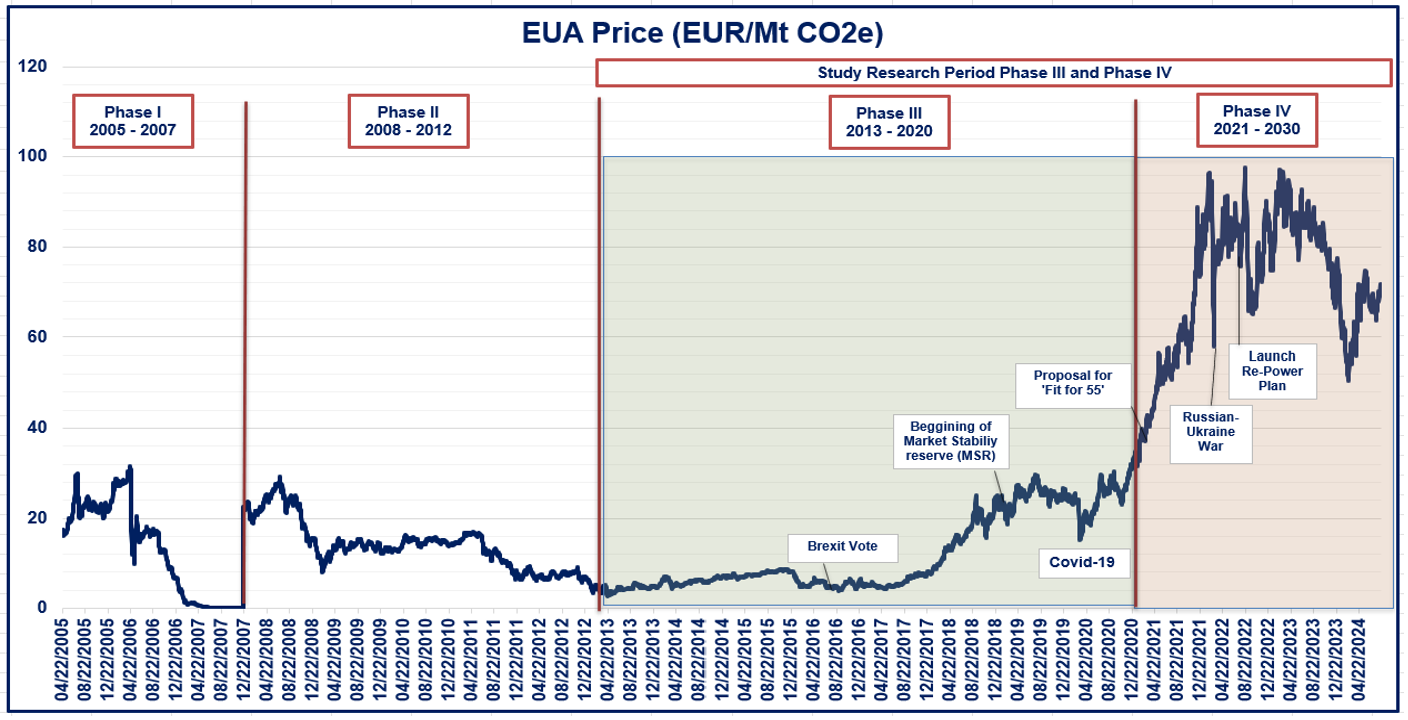
\includegraphics[width = \textwidth]{../figures/1-EUAPrice}
\label{fig:EUAprice}
\end{figure}

For the same period, we also obtain price data for Stoxx 600 Index as a
proxy for the European equity market and the S\&P 500 Index as a proxy
for the International Equity Index. For European sovereign bond markets
we utilize iBoxx Eurozone Sovereign Performance Index, and for European
corporate bond markets we use iBoxx Eur Corporates Index as proxies. To
represent the commodity markets, we additionally obtain the Bloomberg
Metal Commodity Index and the Bloomberg Commodity ex Energy Index, as
energy market exposure is captured separately.

The EUA is represented by the continuous contracts of the most actively
traded financial futures. Given the carbon markets intrinsic
relationship with energy markets, the latter are analyzed independently.
Specifically, we use continuous futures contracts for Brent crude oil,
API2 Rotterdam coal, and TTF natural gas as proxies for the Europeal
oil, coal, and gas markets, respectively. In total, this data set
comprises of 30,140 observations. All prices are converted to EUR to
eliminate the impact of currency fluctuations. Returns are
log-normalized, and volatilities are estimated based on a rolling window
of 20-day daily returns.

Table \ref{table:descriptivestats} provides the descriptive statistics
of daily returns in panel (a) and volatility in panel (b). Both panels
show that all variables are skewed and leptokurtic. Together with
Jarque-Bera that strongly rejects the null hypothesis of a normal
distribution, it is evident that none of the variables conform to a
normal distribution.\\

\begin{table}[htpb]
  \caption{Descriptive statistics of daily return and volatility}
  \label{table:descriptivestats}
   \begin{adjustbox}{width=1\textwidth}
    \begin{tabular}{|l|c|c|c|c|c|c|c|c|c|c|} 
    \multicolumn{11}{@{}l}{\em(a) Daily logarithmic return}\\ \hline
          & Mean & Median & Max & Min & St.Dev. & Skewness & Kurtosis & Obs. & J-B & Prob. \\ \hline
        CARBON & 0.0013 & 0.0008 & 0.2690 & -0.3508 & 0.0311 & -0.2896 & 10.6147 & 3011 & 14177.78 & 0 \\ \hline
        EUROSTOXX & 0.0003 & 0.0006 & 0.0840 & -0.1148 & 0.0099 & -0.8462 & 11.3898 & 3011 & 16634.71 & 0 \\ \hline
        BRENTOIL & 0.0002 & 0.0008 & 0.2224 & -0.2483 & 0.0230 & -0.1878 & 14.1649 & 3011 & 25190.26 & 0 \\ \hline
        COALAPI & 0.0005 & 0.0000 & 0.5935 & -0.2571 & 0.0274 & 3.2819 & 98.0915 & 3011 & 1212557 & 0 \\ \hline
        NATGAS & 0.0009 & -0.0001 & 0.5034 & -0.2983 & 0.0401 & 1.2270 & 17.3396 & 3011 & 38475.98 & 0 \\ \hline
        EURSOVER & 0.0001 & 0.0001 & 0.0200 & -0.0171 & 0.0030 & 0.1270 & 4.3384 & 3011 & 2369.475 & 0 \\ \hline
        EURCORP & 0.0001 & 0.0001 & 0.0137 & -0.0218 & 0.0019 & -0.6075 & 12.0755 & 3011 & 18479.1 & 0 \\ \hline
        SPXINDEX & 0.0006 & 0.0006 & 0.1032 & -0.1260 & 0.0114 & -0.4644 & 13.8660 & 3011 & 24229.62 & 0 \\ \hline
        COMEXENG & 0.0000 & 0.0000 & 0.0407 & -0.0396 & 0.0072 & -0.0775 & 2.1079 & 3011 & 560.4679 & 0 \\ \hline
        METALS & 0.0001 & 0.0000 & 0.0599 & -0.0969 & 0.0101 & -0.3869 & 6.4988 & 3011 & 5373.834 & 0 \\ \hline
    \end{tabular}
    \end{adjustbox}
    
\bigskip
    \ \begin{adjustbox}{width=1\textwidth}
    \begin{tabular}{|l|c|c|c|c|c|c|c|c|c|c|} 
    \multicolumn{11}{@{}l}{\em(b) Volatility}\\ \hline
          & Mean & Median & Max & Min & St.Dev. & Skewness & Kurtosis & Obs & J-B & Prob. \\ \hline
        CARBON & 0.4402 & 0.3916 & 1.8455 & 0.1317 & 0.2265 & 2.2435 & 7.7022 & 3014 & 9978.411 & 0 \\ \hline
        EUROSTOXX & 0.1383 & 0.1223 & 0.7035 & 0.0315 & 0.0753 & 2.8685 & 13.9645 & 3014 & 28623.02 & 0 \\ \hline
        BRENTOIL & 0.3151 & 0.2732 & 1.6611 & 0.0772 & 0.1852 & 2.7509 & 10.9659 & 3014 & 18903 & 0 \\ \hline
        COALAPI & 0.3135 & 0.2241 & 2.6857 & 0.0000 & 0.2985 & 3.7413 & 20.9101 & 3014 & 61940.62 & 0 \\ \hline
        NATGAS & 0.4863 & 0.3490 & 3.1750 & 0.0506 & 0.4070 & 2.2835 & 8.3829 & 3014 & 11444.49 & 0 \\ \hline
        EURSOVER & 0.0422 & 0.0354 & 0.1337 & 0.0129 & 0.0223 & 1.5943 & 2.5774 & 3014 & 2111.037 & 0 \\ \hline
        EURCORP & 0.0248 & 0.0189 & 0.1130 & 0.0071 & 0.0154 & 2.1823 & 5.9139 & 3014 & 6784.517 & 0 \\ \hline
        SPXINDEX & 0.1546 & 0.1306 & 1.0152 & 0.0574 & 0.0942 & 4.7283 & 34.8012 & 3014 & 163327.9 & 0 \\ \hline
        COMEXENG & 0.1080 & 0.1010 & 0.3428 & 0.0460 & 0.0373 & 2.1601 & 7.9794 & 3014 & 10339.95 & 0 \\ \hline
        METALS & 0.1476 & 0.1343 & 0.4863 & 0.0482 & 0.0624 & 1.7810 & 4.8952 & 3014 & 4602.693 & 0 \\ \hline
    \end{tabular}
    \end{adjustbox}
\end{table}

Following previous studies
\citep{diebold_better_2012, reboredo_volatility_2014, gabauer_dynamic_2021}
we transform the data with logarithmic returns and 20-day volatility of
logarithmic returns.

For connectedness analysis, it is also essential that the time series
data are stationary \citep{diebold_better_2012, zhang_oil_2017}. To test
for stationarity, we employ Augmented Dickey-Fuller (ADF)
\citep{dickey_distribution_1979} and Phillips-Perron (PP)
\citep{phillips_testing_1988} tests. Both tests strongly reject the null
hypothesis for a presence of a unit root in either returns
\((p = 0.000)\) or volatility data \((p=0.000)\), suggesting that they
are both stationary.

\hypertarget{empirical-results}{%
\section{Empirical Results}\label{empirical-results}}

\hypertarget{static-total-connectedness}{%
\subsection{Static Total
Connectedness}\label{static-total-connectedness}}

We first investigate the total spillover. Table \ref{table:staticsm}
Panel (a) illustrates the static connectedness of returns while panel
(b) shows the same for volatility between EUAs and other markets. The
full table is in \ref{appendix:a}. The Total Connected Indices (TCIs)
are at 45.19\% for returns and 48.62\% for volatility, respectively,
indicating a moderate level of connectedness across all markets since
this implies that the remainder 54.81\% of the market return and 51.38\%
of the volatility variations across the entire system can be attributed
to idiosyncratic shocks and market-specific factors, i.e.~factors that
impact one market but not others.

The static directional spillovers indicate that the EUAs contribute
34.82\% to the returns of other markets and 31.25\% to their volatility
while receiving from other markets 38.56\% and 43.2\% return and
volatility shocks, respectively. Accordingly, the EUAs are net return
receiver of 3.74\% and volatility spillover receiver of 11.94\%. This
also means that the remaining 61.44\% of the return and 56.8\% of the
volatility in EUAs are explained by its own specific market factors.
Overall, the results seem to suggest a relatively low integration of
EUAs with other markets, although they appear to be somewhat influenced
by the return and volatility of these other markets.

\begin{table}[ht]
  \caption{Static Return and Volatility Connectedness Matrix (Jan 2013 - Aug 2024)}
  \label{table:staticsm}
  \parbox{.5\linewidth}{
    \centering
    \begin{tabular}{|l|l|l|}
    \multicolumn{3}{@{}l}{\em(a) Carbon returns connectedness matrix}\\ \hline
       & CARBON & DSF (FROM) \\ \hline
       CARBON & 61.44 & \textbf{38.56} \\ \hline
       DST (TO) & \textbf{34.82} & 451.90 \\ \hline
       Inc.Own & 96.26 & \textbf{TCI} \\ \hline
       NS (NET) & \textbf{-3.74} & \textbf{45.19} \\ \hline
    \end{tabular}
  }
  \parbox{.5\linewidth}{
    \centering
    \begin{tabular}{|l|l|l|} 
    \multicolumn{3}{@{}l}{\em(b) Carbon volatility connectedness matrix}\\ \hline
       & CARBON & DSF (FROM) \\ \hline
       CARBON & 56.80 & \textbf{43.20} \\ \hline
       DST (TO) & \textbf{31.25} & 486.15 \\ \hline
       Inc.Own & 88.06 & \textbf{TCI} \\ \hline
       NS (NET) & \textbf{-11.94} & \textbf{48.62} \\ \hline
    \end{tabular}
  }
\end{table}

\hypertarget{dynamic-total-connectedness}{%
\subsection{Dynamic Total
Connectedness}\label{dynamic-total-connectedness}}

The dynamic connectedness showing the variation over time in return
volatility connectedness are plotted in panels (a) and (b) of Figure
\ref{fig:dynTCI}, respectively. This reveals that during period of
financial market stress, such as those triggered by Brexit in 2016,
Covid-19 in 2020, and Russia-Ukraine crisis in 2022, the TCI for both
return and volatility tends to increase, suggesting stronger
connectedness in times of crises, albeit short-lived. In contrast, the
start of Phase IV in 2021 appears in the first instance to have a lesser
impact than these exogenous shocks.

\begin{figure}[H]
  \caption{Dynamic Return and Volatility Connectedness (Jan 2013 – Aug 2024)}
  \label{fig:dynTCI}
      \begin{subfigure}[b]{\textwidth}
        \centering
        \caption{Dynamic return TCI}
        \label{fig:dynretTCI}
        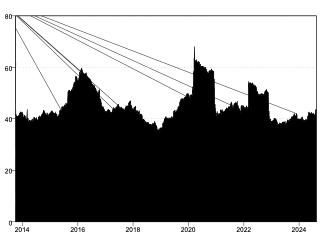
\includegraphics[width = 0.5\linewidth]{../figures/2a-DynRetTCI}
      \end{subfigure}
      \begin{subfigure}[b]{\textwidth}
        \centering
        \bigskip
        \caption{Dynamic volatility TCI}
        \label{fig:dynvolTCI}
        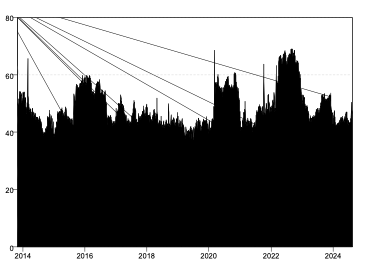
\includegraphics[width = 0.5\linewidth]{../figures/2b-DynVolTCI}
      \end{subfigure}
\end{figure}

Similarly, dynamic net directional connectedness of EUAs with other
markets are provided in Figure \ref{fig:NDC} (\ref{appendix:b} provides
the complete set of charts). These also suggest that in periods of
financial stress the return and volatility connectedness between the
EUAs and other markets increase, supporting the implications derived
from the dynamic TCIs. Importantly, in contrast to the EUAs net return
connectedness in panel (a) that shows EUAs as a receiver of return
shocks from other markets, panel (b) shows that the volatility net
connectedness briefly flips to positive in times of financial stress.

\begin{figure}[H]
  \caption{Net Directional Connectedness between EUAs and other markets}
  \label{fig:NDC}
      \begin{subfigure}[b]{\textwidth}
      \centering
        \caption{Dynamic return net directional connectedness}
        \label{fig:dynretNDC}
        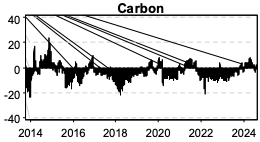
\includegraphics[width = 0.45\linewidth]{../figures/3a-DynRetNDC}
      \end{subfigure}
      \begin{subfigure}[b]{\textwidth}
        \centering
        \bigskip
        \caption{Dynamic volatility net directional connectedness}
        \label{fig:dynvolNDC}
        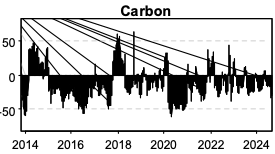
\includegraphics[width = 0.45\linewidth]{../figures/3b-DynVolNDC}
      \end{subfigure}
\end{figure}

\bigskip

\hypertarget{static-pairwise-connectedness}{%
\subsection{Static Pairwise
Connectedness}\label{static-pairwise-connectedness}}

TCI results are informative. However, as Section 3 highlighted, for
networks with more than two variables, TCI tends to be less efficient
and accurate than PCI. PCI measures the level of connectedness between
two specific markets and quantifies how much the return or volatility
variation in one market is impacting, or being impacted by, the other
market. Figure 4 illustrates the network representation of PCI where a
line between markets means that a pairwise connectedness exists between
them. The thickness of the lines indicates the magnitude of such
connectedness. For example, in panel (a) a strong pairwise connectedness
exists between European sovereign and corporate bond returns, whereas
such a pairwise connectedness between coal and natural gas returns is
weaker, and between either of the European bonds and coal returns is
inexistent. Panel (b) displays a similar interpretation for volatility
connectedness.

The PCI return connectedness network in panel (a) suggests that EUAs
(Carbon) seem to operate as an independent market, exhibiting pair
connectedness only with coal and natural gas, where there is also an
equally weak pairwise connection between coal and natural gas. These
could be attributed to fuel switching in the power sector. Coal-to-gas
switching in the European energy market is a function of relative carbon
and fuel costs, driven by the EU ETS and fluctuating commodity prices.
As EUA prices rise the marginal cost of CO2 emissions increases,
impacting coal particularly due to its higher carbon intensity. This
cost differential incentivizes a shift towards gas-fired generation,
which emits roughly half the CO2 per unit of energy, creating a link
between these markets. However, the elasticity of this switch is
contingent on natural gas prices. When gas prices escalate the cost
advantage of switching diminishes, potentially leading utilities to
revert to coal despite the higher carbon costs, thereby increasing EUA
demand and exerting upwards pressure on EUA prices. Therefore,
fluctuations in natural gas or coal prices can alter the economic
attractiveness of this fuel switch, further reinforcing the
connectedness. This would support the findings of
\citet{bertrand_carbon_2014}, \citet{hintermann_allowance_2010},
\citet{creti_carbon_2012}, and \citet{pettersson_fuel_2012} among
others.

The PCI volatility network in panel (b) reveals similar patterns, though
EUAs demonstrate volatility linkages with natural gas exclusively, and
not with coal. This observation is supported by the findings of
\citet{falbo_renewables_2019} and \citet{bertrand_carbon_2014}, who
argue that various EU initiatives and policies aimed at increasing the
share of renewables in the power grid have led to EUAs being more
closely linked with natural gas rather than coal. This connection
appears to persist despite a brief shift back to coal during 2022,
driven by the energy crisis caused by the Russia-Ukraine war. This
persistence in connections overlaps with RePowerEU Plan which reinforces
and accelerates the increase in share of renewables.

\begin{figure}[H]
  \caption{Network representation of Pairwise Connectedness Index (PCI) (Jan 2013 – August 2024)}
  \label{fig:statPCI}
      \begin{subfigure}[b]{\textwidth}
        \centering
        \caption{Static return PCI network}
        \label{fig:statretPCI}
        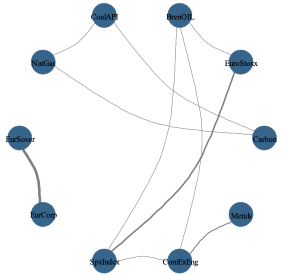
\includegraphics[width = 0.45\linewidth]{../figures/4a-StatRetPCI}
      \end{subfigure}
      \begin{subfigure}[b]{\textwidth}
        \centering
        \bigskip
        \caption{Static volatility PCI network}
        \label{fig:statvolPCI}
        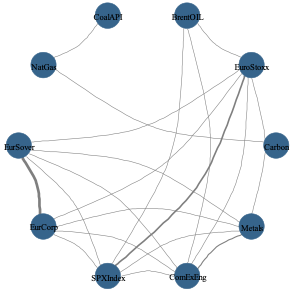
\includegraphics[width = 0.45\linewidth]{../figures/4b-StatVolPCI}
      \end{subfigure}
\end{figure}

\hypertarget{dynamic-pairwise-connectedness}{%
\subsection{Dynamic Pairwise
Connectedness}\label{dynamic-pairwise-connectedness}}

When we examine the return and volatility PCI dynamically over time
(\ref{appendix:c} provides the full set of dynamic PCI charts), we see
in panel (a) of Figure 5 considerable fluctuations in EUAs' pairwise
return connectedness in times of crises. This appears to especially be
the case with EuroStoxx, S\&P 500, brent, coal, and natural gas which
all spike to varying degrees around the times of exogenous shocks such
as the Brexit vote in 2016, Covid-19 crisis in 2020, and Russia-Ukraine
war in 2022. A similar behavior is observed, albeit to a lesser extent,
with sovereign and corporate bonds, metals and other commodities during
these shocks. As we have hypothesized, most of these are short-lived and
it appears that coal and natural gas have some return connectedness with
the EUAs over time.

There also seems to be an increase in the return connectedness between
EUAs and natural gas, while a decrease with coal, especially from 2021
onwards. These changes can be attributable to various market,
regulatory, and policy factors such as the introduction of Phase IV and
impact of RePowerEU which is accelerating the deployment of renewable
energy across Europe, helping the EU advance its climate goals and
reduce greenhouse gas emissions, while also diminishing reliance on
Russian energy imports \citep{repowereu_2024}. Changes in the energy
mix, with a shift towards a relatively cleaner energy sources including
natural gas under the EU's climate targets and the Fit for 55 package
can influence the demand for and price of EUAs, thus increasing their
connectedness. Coupling this with the impact of RepowerEU in the
acceleration of renewables capacity can strengthen such influence and
connectedness. Additionally, fluctuations in natural gas prices, due to
factors like supply disruptions or changes in demand, can directly
impact the cost-effectiveness of gas-fired power plants versus coal,
which would also affect the price and demand for EUAs. Furthermore, as
EU member states have been phasing out coal and adopting cleaner energy
sources, thereby reducing the influence of coal prices on the EUAs
market, there has been a regulatory push towards a reduced dependence on
coal, leading to decreased coal usage and a weakened link with EUAs
prices.

Another important observation emerges on the return and volatility
connectedness between carbon and equity markets. While such
connectedness seems inexistent on the static return and volatility PCI
network in panels (a) and (b) of Figure 3, we can observe in the dynamic
return and volatility PCI in panel (a) of Figure 4 that such
connectedness seems to have gained prominence since 2020. A similar
pattern can also be observed in the same panel for EUAs connectedness
with natural gas and metals. Yet, it appears that among all pairwise
connectedness that gained prominence since 2020, only the volatility
connectedness with natural gas is not in a declining trend in that
period.

\begin{figure}[H]
  \caption{Dynamic Return and Volatility Pairwise Connectedness Index (PCI) (Jan 2013 – Aug 2024)}
  \label{fig:dynPCI}
      \begin{subfigure}[b]{\textwidth}
        \centering
        \caption{Dynamic return PCI}
        \label{fig:dynretPCI}
        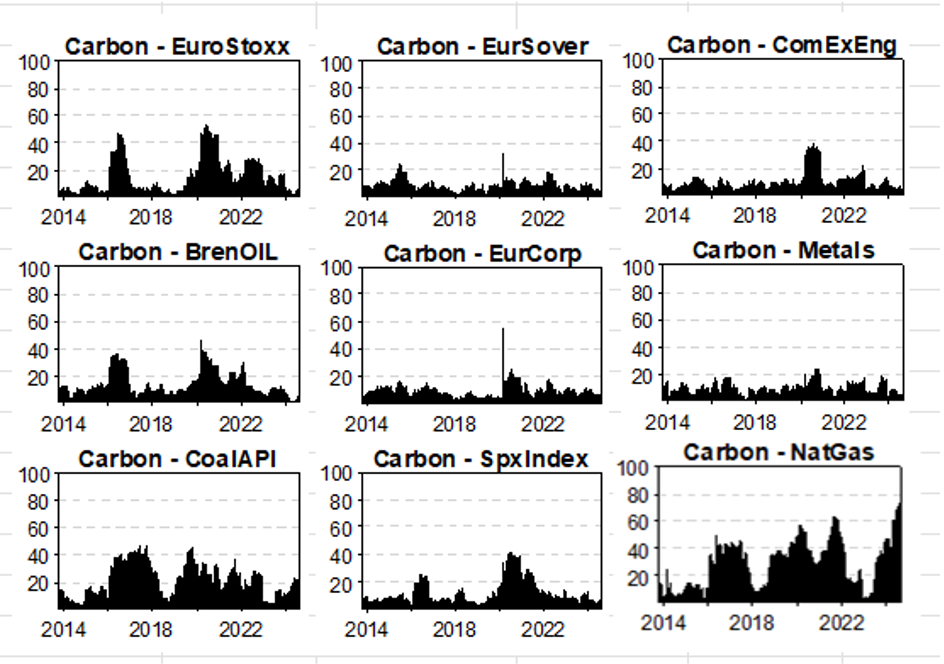
\includegraphics[width = 0.75\textwidth]{../figures/5a-DynRetPCI}
      \end{subfigure}
      \begin{subfigure}[b]{\textwidth}
        \centering
        \bigskip
        \caption{Dynamic volatility PCI network}
        \label{fig:dynvolPCI}
        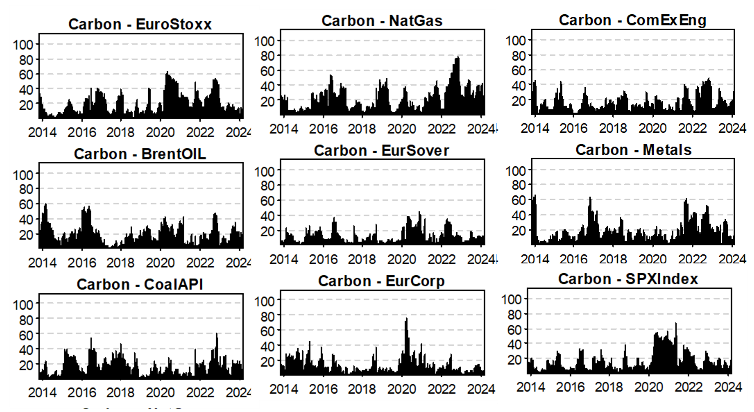
\includegraphics[width = 0.75\textwidth]{../figures/5b-DynVolPCI}
      \end{subfigure}
\end{figure}

Relatively recent introduction of financial products like Exchange
Traded Funds (ETFs) and other investment vehicles focusing on carbon
markets, including EUAs, might be the main contributors to this trend of
strengthened connectedness with the equity markets. These new products
have broadened the participation of financial investors who may be more
responsive to global macroeconomic shifts than specific carbon
fundamentals. This could lead to a strengthening of the return and
volatility linkage between EUAs and equities - a significant finding for
institutional investors looking to integrate EUAs into their portfolios.
Despite this increase in connectedness with equity markets, the results
of this study reveal that the overall interconnectedness of EUAs with
other markets remains relatively low as we hypothesized, reinforcing the
potential diversification benefits of including EUAs in investment
portfolios.

\hypertarget{conclusions}{%
\section{Conclusions}\label{conclusions}}

The EU has set an ambitious climate goal for 2030, committing to achieve
a 55\% reduction in GHG emissions relative to 1990 levels. In order to
meet this objective, the EU has adopted the Fit for 55 package, along
with the RepowerEU Plan. This aligns with a broader objective to
transform the EU into a sustainable economy and establish Europe as a
climate-neutral continent by 2050. A pivotal instrument in EU climate
policy is the EU Emissions Trading System (EU-ETS), a cornerstone
mechanism grounded on a cap-and-trade system that limits and annually
reduces emissions covered by the system. The Fit for 55 package
introduces reforms to the EU-ETS, targeting a more aggressive reduction
in the emission cap for the high-emitting sectors covered by the system.

Various objectives underscore the necessity to tighten the cap, thereby
decreasing the supply of European Emission Allowances (EUAs). To that
end, this study sought to examine the financial characteristics of EUAs
to gain a more comprehensive understanding of this market and explore
whether EUAs can be a market for diversification. We hypothesized that
with the introduction of Phase IV the carbon market will continue to
offer diversification benefits, and that Fit for 55 package and
RePowerEU Plan will engender a longer-lasting linkages with energy
markets. As a result, carbon markets would offer diversification
benefits that would likely to be more pronounced for non-energy
portfolios. We also hypothesized that in times of exogenous shocks,
carbon may link with other asset classes, though in shorter duration. To
test our hypothesis, we have adopted an econometric model of
connectedness analysis.

Our findings showed that despite an observed increase in the
connectedness of EUAs with other financial markets---particularly during
periods of financial stress---EUAs remain largely independent from these
markets, except for coal and natural gas. A natural connection with
these energy commodities exists due to significant participation of
power generation in the EU-ETS. Overall, the results suggest that the
return and volatility behavior of EUAs are primarily driven by their own
fundamental factors. For investors, it suggests that EUAs could offer
potential diversification benefits when included in a portfolio, due to
their low linkage and spillover effect with other markets. We recommend,
for future research, investigating the behavior of non-energy and broad
market portfolios when carbon is incorporated at various densities in
order to empirically ascertain the magnitude of potential
diversification benefits this asset class offers. For policy makers, the
results of the connectedness between EUAs and other markets can provide
valuable insights. They can, for example, adopt a systemic view in
considering the impacts on various markets when developing energy and
climate policies. This would help in ensuring that the response of these
markets to such policies are not only supportive but even help in
accelerating the realization of these policy objectives. Accordingly,
for future research, we recommend investigating the potential behaviors
of various markets through connectedness analysis in response to broader
sustainability policies the EU or other jurisdictions are considering.

\newpage

\appendix
\section{Static Return and Volatility Connectedness Matrix}
\label{appendix:a}
  \begin{table}[H]
    \caption{Static Return and Volatility Connectedness Matrix (Jan 2013 - Aug 2024)}
    \label{table:staticfull}
    \begin{adjustbox}{width=1.1\textwidth}
      \begin{tabular}{|l|c|c|c|c|c|c|c|c|c|c|c|} 
        \multicolumn{12}{@{}l}{\em(a) Carbon returns connectedness matrix}\\ \hline
      & CARBON & EUROSTOXX & BRENTOIL & COALAPI & NATGAS & EURSOVER & EURCORP & SPXINDEX & COMEXENG & METALS & DSF (FROM) \\ \hline
       CARBON & 61.44 & 4.10 & 3.87 & 6.63 & 9.94 & 2.50 & 2.21 & 3.6 & 2.68 & 2.96 & \textbf{38.56} \\ \hline
       EUROSTOXX & 3.54 & 49.47 & 5.83 & 3.10 & 3.09 & 3.09 & 3.58 & 19.99 & 5.27 & 3.04 & 50.53 \\ \hline
       BRENTOIL & 3.72 & 6.17 & 57.92 & 4.40 & 3.74 & 2.56 & 2.20 & 7.39 & 8.37 & 3.52 & 42.08 \\ \hline
       COALAPI & 6.17 & 3.94 & 5.33 & 59.58 & 10.81 & 1.84 & 1.91 & 3.97 & 3.84 & 2.60 & 40.42 \\ \hline
       NATGAS & 9.91 & 3.00 & 4.05 & 10.23 & 61.68 & 1.95 & 1.86 & 2.51 & 2.59 & 2.21 & 38.32 \\ \hline
       EURSOVER & 1.96 & 2.96 & 2.54 & 1.51 & 1.74 & 48.65 & 31.77 & 2.37 & 1.98 & 4.52 & 51.35 \\ \hline
       EURCORP & 2.01 & 5.17 & 2.68 & 1.87 & 1.87 & 30.07 & 45.48 & 3.98 & 2.47 & 4.40 & 54.52 \\ \hline
       SPXINDEX & 2.49 & 18.09 & 7.00 & 3.26 & 2.02 & 2.42 & 2.71 & 53.19 & 6.42 & 2.40 & 46.81 \\ \hline
       COMEXENG & 2.63 & 5.16 & 7.57 & 3.32 & 2.51 & 2.18 & 2.37 & 6.70 & 53.24 & 14.31 & 46.76 \\ \hline
       METALS & 2.38 & 3.08 & 3.19 & 2.24 & 2.50 & 4.94 & 5.65 & 2.91 & 15.66 & 57.45 & 42.55 \\ \hline
       DST (TO) & \textbf{34.82} & 51.76 & 42.07 & 36.56 & 38.21 & 51.55 & 54.27 & 53.42 & 49.29 & 39.95 & 451.90 \\ \hline
       Inc.Own & 96.26 & 101.23 & 99.99 & 96.14 & 99.89 & 100.20 & 99.75 & 106.61 & 102.53 & 97.40 & \textbf{TCI} \\ \hline
       NS (NET) & \textbf{-3.74} & 1.23 & -0.01 & -3.86 & -0.11 & 0.20 & -0.25 & 6.61 & 2.53 & -2.60 & \textbf{45.19} \\ \hline
      \end{tabular}
    \end{adjustbox}
    
\bigskip\bigskip
    \begin{adjustbox}{width=1.1\textwidth}
        \begin{tabular}{|l|c|c|c|c|c|c|c|c|c|c|c|} 
          \multicolumn{12}{@{}l}{\em(b) Carbon volatility connectedness matrix}\\ \hline
       & CARBON & EUROSTOXX & BRENTOIL & COALAPI & NATGAS & EURSOVER & EURCORP & SPXINDEX & COMEXENG & METALS & DSF (FROM) \\ \hline
       CARBON & 56.80 & 4.66 & 4.45 & 6.41 & 7.17 & 3.41 & 3.40 & 4.77 & 4.19 & 4.74 & \textbf{43.20} \\ \hline
       EUROSTOXX & 3.80 & 47.26 & 4.87 & 3.81 & 3.69 & 5.09 & 4.15 & 16.18 & 5.36 & 5.82 & 52.74 \\ \hline
       BRENTOIL & 4.35 & 6.78 & 51.50 & 4.50 & 4.17 & 3.98 & 4.67 & 6.92 & 7.19 & 5.94 & 48.50 \\ \hline
       COALAPI & 4.53 & 3.91 & 3.56 & 61.61 & 7.36 & 3.03 & 2.59 & 4.79 & 3.42 & 5.20 & 38.39 \\ \hline
       NATGAS & 4.58 & 4.70 & 3.61 & 7.84 & 58.94 & 3.87 & 4.31 & 4.74 & 3.76 & 3.66 & 41.06 \\ \hline
       EURSOVER & 1.83 & 6.07 & 3.51 & 2.47 & 2.19 & 44.66 & 25.24 & 5.73 & 3.73 & 4.57 & 55.34 \\ \hline
       EURCORP & 2.52 & 5.79 & 2.43 & 2.56 & 2.46 & 27.69 & 42.37 & 6.36 & 4.48 & 3.34 & 57.63 \\ \hline
       SPXINDEX & 3.22 & 15.05 & 4.92 & 2.89 & 1.80 & 4.78 & 3.90 & 53.70 & 4.55 & 5.21 & 46.30 \\ \hline
       COMEXENG & 2.80 & 7.84 & 4.64 & 3.97 & 4.49 & 5.51 & 5.54 & 6.94 & 48.77 & 9.52 & 51.23 \\ \hline
       METALS &3.63 & 8.27 & 4.06 & 4.33 & 4.55 & 5.17 & 6.35 & 6.12 & 9.28 & 48.24 & 51.76 \\ \hline
       DST (TO) & \textbf{31.25} & 63.05 & 36.04 & 38.77 & 37.87 & 62.53 & 60.15 & 62.53 & 45.95 & 48.00 & 486.15 \\ \hline
       Inc.Own & 88.06 & 110.31 & 87.54 & 100.39 & 96.81 & 107.19 & 102.52 & 116.23 & 94.72 & 96.24 & \textbf{TCI} \\ \hline
       NS (NET) & \textbf{-11.94} & 10.31 & -12.46 & 0.39 & -3.19 & 7.19 & 2.52 & 16.23 & -5.28 & -3.76 & \textbf{48.62} \\ \hline
      \end{tabular}
    \end{adjustbox}
\end{table}

\section{Dynamic Return and Volatility Net Directional Connectedness}
\label{appendix:b}
\begin{figure}[H]
  \caption{Dynamic Net Directional Connectedness (Jan 2013 – Aug 2024)}
  \label{fig:dynNDCfull}
      \begin{subfigure}[H]{\textwidth}
        \centering
        \caption{Dynamic return net directional connectedness}
        \label{fig:dynretNDCfull}
        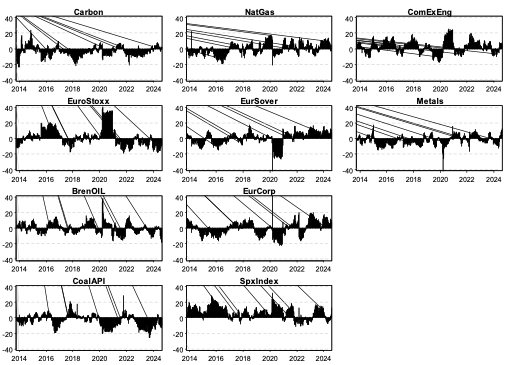
\includegraphics[width =\textwidth]{../figures/6a-AppBa-DynRetNDCfull}
      \end{subfigure}
    \bigskip
      \begin{subfigure}[H]{\textwidth}
        \centering
        \caption{Dynamic volatility net directional connectedness}
        \label{fig:dynvolNDCfull}
        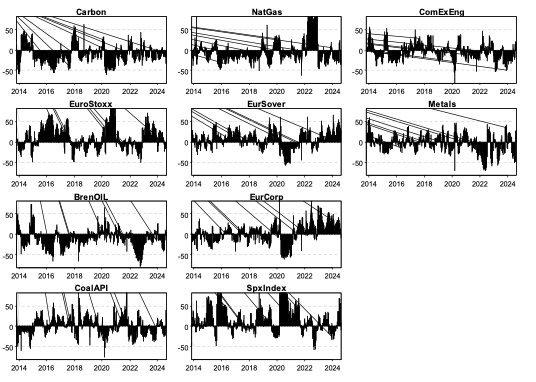
\includegraphics[width = \textwidth]{../figures/6b-AppBb-DynVolNDCfull}
      \end{subfigure}
\end{figure}

\section{Dynamic Return and Volatility Pairwise Connectedness Index}
\label{appendix:c}
\begin{figure}[H]
  \caption{Dynamic Return and Volatility Pairwise Connectedness Index (Jan 2013 – Aug 2024)}
  \label{fig:dynPCIfull}
      \begin{subfigure}[H]{\textwidth}
        \centering
        \caption{Dynamic return PCI}
        \label{fig:dynretPCIfull}
        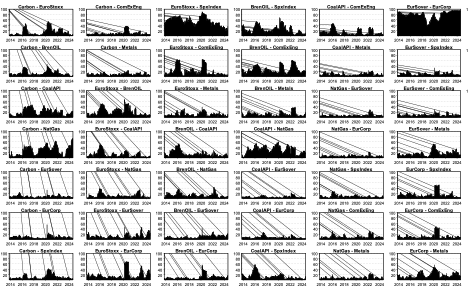
\includegraphics[width = \textwidth]{../figures/7a-AppCa-DynRetPCIfull}
      \end{subfigure}
    \bigskip
      \begin{subfigure}[H]{\textwidth}
        \centering
        \caption{Dynamic volatility PCI}
        \label{fig:dynvolPCIfull}
        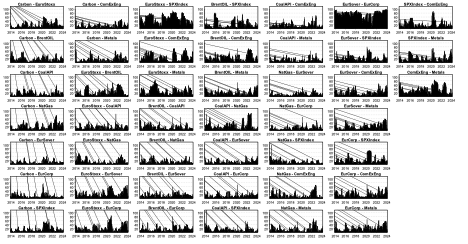
\includegraphics[width = \textwidth]{../figures/7b-AppCa-DynVolPCIfull}
      \end{subfigure}
\end{figure}

\renewcommand\refname{References}
\bibliography{EUAbibliography.bib}


\end{document}
